\documentclass[10pt]{article}
% Submission (anonymous): \usepackage{tmlr}.  Named preprint: \usepackage[preprint]{tmlr}.
\usepackage[preprint]{tmlr}
\usepackage[T1]{fontenc}
\usepackage{amsmath,amssymb}
\usepackage{booktabs}
\usepackage{graphicx}
\usepackage{hyperref}
\usepackage{url}
\usepackage{xcolor}
\newcommand{\PENDING}[1]{\textcolor{red}{[PENDING: #1]}}

\title{GreenLight: Synthetic Patient Data for the Early Weeks of an Outbreak, Built from Past Diseases and Released Only When Ready}

\author{\name Author Name \email author@example.com \\
      \addr Independent researcher}

\def\month{MM}
\def\year{YYYY}
\def\openreview{\url{https://openreview.net/forum?id=XXXX}}

\begin{document}
\maketitle

\begin{abstract}
In the first weeks of a new outbreak, too few patients have known outcomes to train a reliable model of who dies,
yet decisions and data sharing cannot wait. A natural idea is to borrow from earlier outbreaks, to say when the
borrowed model is ready, and only then to release synthetic patient records. We build such a system, GreenLight, and evaluate it the way it would be used, on OutbreakReplay: a benchmark that
replays 32 real outbreaks of hospitalised severe acute respiratory illness from Brazil's public surveillance (2.5 million patients, 2013--2025) day by day, never using
information from the future. Four findings stand out. (1)~Using each patient's final outcome from the day the record
was entered, a common shortcut, inflates early accuracy enough to reverse a conclusion: on day 28 of COVID-19 in 2020
only 32\% of the outcomes so used were known, and GreenLight's apparent advantage over real data alone disappeared once this
was fixed. (2)~In a pre-registered test on nine unseen seasons (2023--2025), simply pooling earlier seasons was
\emph{more} accurate than GreenLight and every adaptive borrowing method, and came within 0.001 AUC of a hindsight reference
without any current data. (3)~A stability-based readiness signal was honest (one borderline false signal in 31
outbreaks), whereas a standard minimum-sample-size rule declared readiness within 90 days in only 8 of 32
outbreaks, and never for other respiratory viruses. (4)~Synthetic data released at that signal trained better models than the real records it was built
from and than five standard generators trained on those records, because it carries borrowed knowledge. We report
the negative result as found and release code to reproduce every number.
\end{abstract}

\section{Introduction}
When a respiratory pathogen causes a new wave of hospitalisations, the clinical question ``who is likely to die?''
arises long before the outbreak's own data can answer it. In the first weeks, few patients have been admitted and
fewer have a known outcome. Models trained on these records alone are unstable, and the many COVID-19 prognostic
models built from small early samples were mostly at high risk of bias \citep{wynants2020covid}. Sharing patient
records to pool evidence is slow, so synthetic patient data are often proposed as a stop-gap.

Three questions follow, and they are rarely studied together. \emph{Can earlier outbreaks help?} Transfer from
earlier diseases has worked for COVID-19 outcome prediction \citep{lichtner2021covid,agarwal2022transmed}, and
clinical-trial statistics offers a family of ways to borrow from historical data
\citep{ibrahim2000power,hobbs2011commensurate,schmidli2014rmap,kaizer2018mem}. \emph{When is a model ready?}
Minimum sample sizes exist for models developed on one's own data \citep{riley2020samplesize}, but not for a model
that borrows. \emph{Is synthetic data released early useful?} Generators trained on a few hundred records can only
reproduce what those records contain.

We study all three on real data, under the conditions a health agency would face. Our contributions:
\begin{enumerate}
\item \textbf{OutbreakReplay, a time-respecting replay benchmark} over 32 outbreaks (influenza, other respiratory viruses and
COVID-19) from public Brazilian surveillance, in which every method sees, each day, only the records entered so far
and only the outcomes known so far (Section~\ref{sec:setup}).
\item \textbf{GreenLight}, an interpretable system that votes on which earlier outbreaks the new one
resembles, borrows from them with a strength that fades as its own data grow, falls back to a safe age rule when
the pathogen is new, signals when its model is ready (it gives the \emph{green light}), and only then releases labelled
synthetic data (Section~\ref{sec:os}).
\item \textbf{A careful evaluation}: 9 borrowing baselines, 5 synthetic-data generators, a sample-size readiness
rule, intervals at the patient and outbreak level, and a final test on nine seasons that were downloaded only after
the plan, settings and analysis code were committed (Section~\ref{sec:results}).
\end{enumerate}
Our main empirical findings are summarised in the abstract. Two are negative or cautionary: ignoring when outcomes
become known can reverse conclusions, and on familiar seasons with a rich history, plain pooling beats adaptive
borrowing. We think both are useful to anyone evaluating early-outbreak models.

\section{Related work}
\paragraph{Borrowing from historical data.} Power priors \citep{ibrahim2000power}, commensurate priors
\citep{hobbs2011commensurate}, robust meta-analytic-predictive priors \citep{schmidli2014rmap} and multi-source
exchangeability models \citep{kaizer2018mem} decide how much to trust historical or supplementary data. GreenLight's
borrowing rule is a simple member of this family; we include representatives of each as baselines.
\paragraph{Transfer and meta-learning for clinical prediction.} Transfer learning \citep{pan2010transfer} from
non-COVID viral pneumonia \citep{lichtner2021covid} and from severe respiratory admissions
\citep{agarwal2022transmed} improved COVID-19 outcome prediction; MetaPred meta-learns across related clinical
tasks \citep{zhang2019metapred}. Borrowing from the wrong source can hurt (negative transfer,
\citealp{wang2019negative}). These studies evaluate one fixed transfer at one time; we evaluate day by day, with a
choice among many sources.
\paragraph{Readiness.} \citet{riley2020samplesize} give the minimum sample size for developing a prediction model
with acceptable overfitting and precision. We compare it with our stability-based green light.
\paragraph{Real-time severity and reporting delay.} Early case-fatality estimates are biased because recent cases
have not yet resolved \citep{nishiura2009cfr}, and nowcasting corrects counts for reporting delay
\citep{hohle2014nowcasting}. We show the analogous problem for patient-level machine-learning replays.
\paragraph{Synthetic tabular data.} CTGAN and TVAE \citep{xu2019ctgan}, TabDDPM \citep{kotelnikov2023tabddpm},
adversarial random forests \citep{watson2023arf} and Bayesian networks, available in synthcity
\citep{qian2023synthcity}, are standard generators. Synthetic data are not automatically private
\citep{stadler2022groundhog}; our data are public, and we report a simple copy check.

\section{Data and the OutbreakReplay protocol}\label{sec:setup}
\paragraph{Data.} SIVEP-Gripe, Brazil's national surveillance of hospitalised severe acute respiratory illness, is
published by the Ministry of Health under CC-BY \citep{srag_data}. We use hospitalised patients with a recorded
outcome (cure or death), the H1N1 pandemic of 2009 and the years 2013--2025. An \emph{outbreak} is one file year and
laboratory class: influenza, other respiratory virus, or COVID-19 (from 2020). Features are those the admission form
collects in every year: age, sex, self-reported race, state, six symptoms and ten conditions (yes / no / missing).
The development set has 24 outbreaks (2009--2022; 2.14 million patients), 23 of which have an earlier outbreak to
borrow from; the frozen test set has 9 (2023--2025; 0.37 million). Table~\ref{tab:data} describes each outbreak.

\begin{table}[t]
\centering\scriptsize
\caption{Outbreaks. Patients: hospitalised with a recorded outcome. Missing: share of the 16 yes/no fields not collected or not filled in. Day 0: start of the replay. Test: patients admitted on days 91--182 (July 2020 for COVID-19 2020). Green: GreenLight's green-light day ($-$: none by day 90). H1N1 2009 is used only as an earlier outbreak to borrow from.}\label{tab:data}
\resizebox{\linewidth}{!}{%
\begin{tabular}{llrrrrlrrr}
\toprule
Set & Outbreak & Patients & Died (\%) & Median age & Missing (\%) & Day 0 & Test patients & Test deaths & Green \\
\midrule
Development & Influenza 2013 & 6,146 & 16.2 & 35 & 7 & 2013-04-02 & 2,483 & 371 & 70 \\
 & Other virus 2013 & 3,120 & 7.1 & 1 & 6 & 2013-04-10 & 1,046 & 85 & $-$ \\
 & Influenza 2014 & 1,762 & 18.6 & 36 & 8 & 2014-04-01 & 751 & 135 & 46 \\
 & Other virus 2014 & 2,249 & 5.7 & 1 & 5 & 2014-03-25 & 792 & 33 & 34 \\
 & Influenza 2015 & 1,257 & 16.2 & 39 & 6 & 2015-03-09 & 579 & 96 & 36 \\
 & Other virus 2015 & 2,418 & 5.0 & 1 & 6 & 2015-02-23 & 1,129 & 60 & 64 \\
 & Influenza 2016 & 11,824 & 18.8 & 39 & 6 & 2016-02-12 & 3,896 & 849 & 32 \\
 & Other virus 2016 & 4,607 & 6.6 & 1 & 4 & 2016-03-07 & 2,412 & 154 & 70 \\
 & Influenza 2017 & 3,255 & 15.2 & 44 & 4 & 2017-02-01 & 1,577 & 225 & 24 \\
 & Other virus 2017 & 4,689 & 6.4 & 1 & 4 & 2017-02-09 & 2,382 & 139 & 46 \\
 & Influenza 2018 & 7,856 & 17.3 & 36 & 4 & 2018-03-01 & 3,973 & 746 & 44 \\
 & Other virus 2018 & 8,071 & 5.8 & 1 & 3 & 2018-01-19 & 4,165 & 239 & 80 \\
 & Influenza 2019 & 6,460 & 17.7 & 36 & 36 & 2019-03-11 & 2,736 & 470 & 12 \\
 & Other virus 2019 & 8,806 & 5.7 & 1 & 46 & 2019-03-08 & 2,264 & 132 & 22 \\
 & COVID-19 2020 & 645,001 & 33.2 & 61 & 42 & 2020-02-26 & 93,626 & 31,426 & 54 \\
 & Influenza 2020 & 2,336 & 13.4 & 34 & 43 & 2020-01-09 & 397 & 75 & 34 \\
 & Other virus 2020 & 4,620 & 7.5 & 3 & 46 & 2020-01-02 & 1,119 & 112 & 38 \\
 & COVID-19 2021 & 1,110,621 & 32.7 & 57 & 46 & 2021-01-01 & 507,241 & 165,882 & 28 \\
 & Influenza 2021 & 10,012 & 15.5 & 59 & 50 & 2021-04-07 & 202 & 26 & 38 \\
 & Other virus 2021 & 19,629 & 3.0 & 1 & 57 & 2021-01-08 & 4,331 & 147 & 50 \\
 & COVID-19 2022 & 214,982 & 27.7 & 70 & 43 & 2022-01-01 & 36,955 & 8,363 & 30 \\
 & Influenza 2022 & 10,826 & 12.6 & 49 & 45 & 2022-01-01 & 1,648 & 176 & 30 \\
 & Other virus 2022 & 31,050 & 2.6 & 1 & 59 & 2022-01-02 & 12,564 & 353 & 42 \\
\midrule
Frozen test & COVID-19 2023 & 44,317 & 19.7 & 68 & 42 & 2023-01-01 & 10,114 & 2,165 & 28 \\
 & Influenza 2023 & 11,196 & 9.6 & 11 & 50 & 2023-01-08 & 7,410 & 747 & 40 \\
 & Other virus 2023 & 46,180 & 2.1 & 1 & 59 & 2023-01-01 & 18,583 & 366 & 52 \\
 & COVID-19 2024 & 27,720 & 18.6 & 68 & 40 & 2024-01-01 & 3,592 & 717 & 34 \\
 & Influenza 2024 & 22,836 & 10.4 & 34 & 46 & 2024-01-03 & 10,798 & 1,179 & 24 \\
 & Other virus 2024 & 61,184 & 2.4 & 1 & 57 & 2024-01-02 & 28,431 & 671 & 38 \\
 & COVID-19 2025 & 15,796 & 16.3 & 61 & 38 & 2025-01-01 & 1,648 & 318 & 32 \\
 & Influenza 2025 & 41,518 & 11.5 & 47 & 41 & 2025-01-01 & 24,959 & 3,359 & 18 \\
 & Other virus 2025 & 97,269 & 2.6 & 1 & 54 & 2025-01-01 & 43,737 & 1,007 & 58 \\
\midrule
Source only & H1N1 2009 & 21,123 & 9.5 & 24 & 47 & -- & -- & -- & -- \\
\bottomrule
\end{tabular}}
\end{table}


\paragraph{Replay.} Each outbreak is replayed from day 0 to day 90 in steps of 2 days. Day 0 is the first record
(COVID-19) or the first week with at least 20 records (seasonal outbreaks). On day $d$ a method may use (i)~records
of the new outbreak (we call it \emph{fob}) entered by day $d$, (ii)~of those, only outcomes \emph{known} by day $d$,
and (iii)~earlier outbreaks' records and outcomes known before fob's day 0. An outcome counts as known from the later
of the entry date and the outcome date (falling back to the case-closure date). Each day's model is scored by AUC on
the patients admitted on days 91--182 (July 2020 for COVID-19 in 2020), which no method sees. Two references:
\emph{gold}, the same model class fitted in hindsight on all of fob's other records, and \emph{rank by age}. The
\emph{gap to gold} is gold's AUC minus the method's.

\section{GreenLight}\label{sec:os}
\paragraph{Kinship Vote.} Each week, every earlier outbreak predicts fob's newly admitted patients: who is
hospitalised (age band, sex and the yes/no fields fob's form collects) and who dies (its severity model with fob's
own death rate). Predictions are scored by log-likelihood, prequentially \citep{dawid1984prequential,gneiting2007scoring}.
A \emph{Stranger} candidate predicts from fob's own earlier weeks. Vote shares are a softmax of accumulated scores
with sharpness $\tau=0.01$, starting from equal shares per pathogen group.
\paragraph{Handover Rule.} The severity model is a MAP logistic regression whose prior mean is the vote-weighted
average of the earlier outbreaks' coefficients and whose strength is $\lambda=10\,(1-s)$, where $s$ is the Stranger's
share; the intercept (fob's own death rate) and the state effects are never borrowed. As fob's records accumulate,
the fixed prior is outweighed and fob's own data take over.
\paragraph{Lab-Label Fallback.} If the laboratory class of fob has no earlier outbreak, GreenLight uses a one-parameter age
trend until 20 deaths have been scored on fresh data, then borrows.
\paragraph{The green light.} GreenLight declares its model ready on day $d$ if at least 10 deaths have a known outcome, the rank
correlation of its risk scores today with those of 8 days earlier is at least 0.99 on two consecutive checks, and GreenLight
is not on the fallback. These two values were re-chosen on the development set after the outcome-timing fix
(Section~\ref{sec:timing}).
\paragraph{Synth Release.} After the green light, GreenLight generates synthetic patients: profiles from a dependency chain
of logistic models (each yes/no field given age band, sex and earlier fields, with priors borrowed as above) and
death drawn from GreenLight's risk model. Every row is labelled synthetic with its provenance.
\paragraph{Glass Box Report.} An HTML page per outbreak and day shows the vote, the risk table with borrowed shares,
the green light conditions and synthetic-versus-real comparisons; examples are in the code repository.

\section{Experiments and results}\label{sec:results}
All settings were chosen on the development set. Intervals are 95\% percentile bootstrap intervals: over outbreaks
(2,000 resamples, paired where methods are compared) or over test patients (1,000 stratified resamples).

\subsection{Outcome timing reverses a conclusion}\label{sec:timing}
Our first replays, like many retrospective evaluations, used each patient's final outcome from the day the record
was entered. For COVID-19 in 2020, on day 28 only 32\% of the outcomes so used, and 35\% of the deaths, had actually
occurred and been recorded (Figure~\ref{fig:timing}). After the fix, the day GreenLight came within 0.02 AUC of gold moved
from 28 to 36, the same as real data alone; GreenLight's apparent COVID-19 advantage was an artefact. On familiar seasons GreenLight
still matched gold from day 0. The fix also produced two false green lights under the original readiness settings,
which we therefore re-chose (Section~\ref{sec:readiness}).

\begin{figure}[t]
\centering
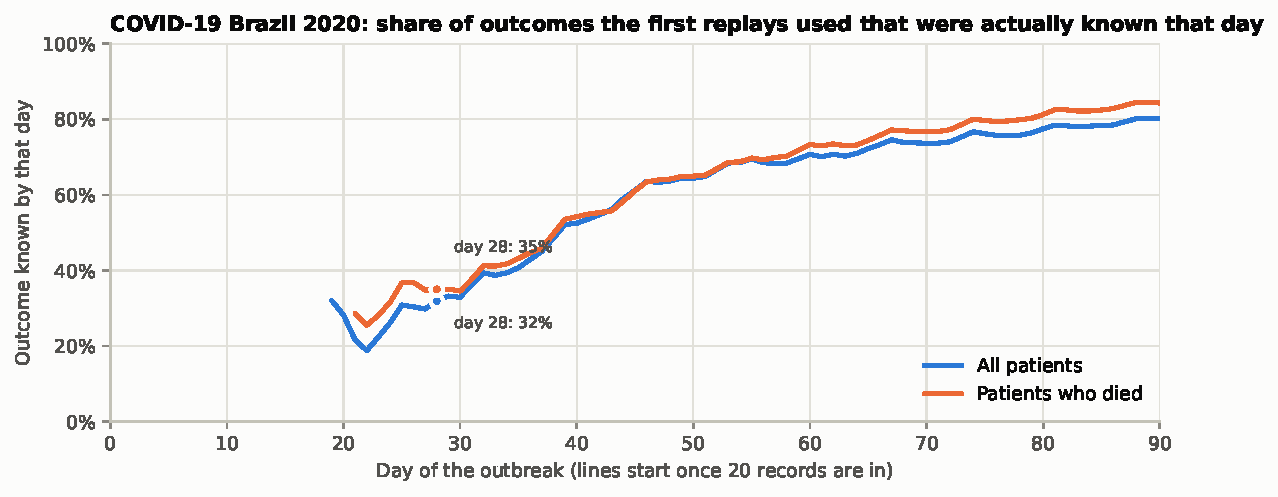
\includegraphics[width=0.85\linewidth]{figures/fig6_outcome_timing.pdf}
\caption{COVID-19, Brazil 2020: share of the outcomes used by an ``outcome on entry'' replay that were actually known
on that day.}\label{fig:timing}
\end{figure}

\subsection{Who dies: borrowing versus baselines}
Figure~\ref{fig:replay} shows typical replays. Table~\ref{tab:baselines} compares GreenLight with nine baselines, all using
the same design and data: a pooled model of earlier outbreaks (no fob data); stacking the pooled earlier outbreaks
with fob's records; fine-tuning towards the pooled model; GreenLight without the vote (equal weights); a meta-analytic prior
and its robust version \citep{schmidli2014rmap}; a borrowing strength chosen by marginal likelihood (commensurate-style,
\citealp{hobbs2011commensurate}); source averaging by marginal likelihood (a simplification of multi-source
exchangeability, \citealp{kaizer2018mem}); and a Reptile meta-learned starting point \citep{nichol2018reptile} in the
spirit of MetaPred \citep{zhang2019metapred}.

\begin{figure}[t]
\centering
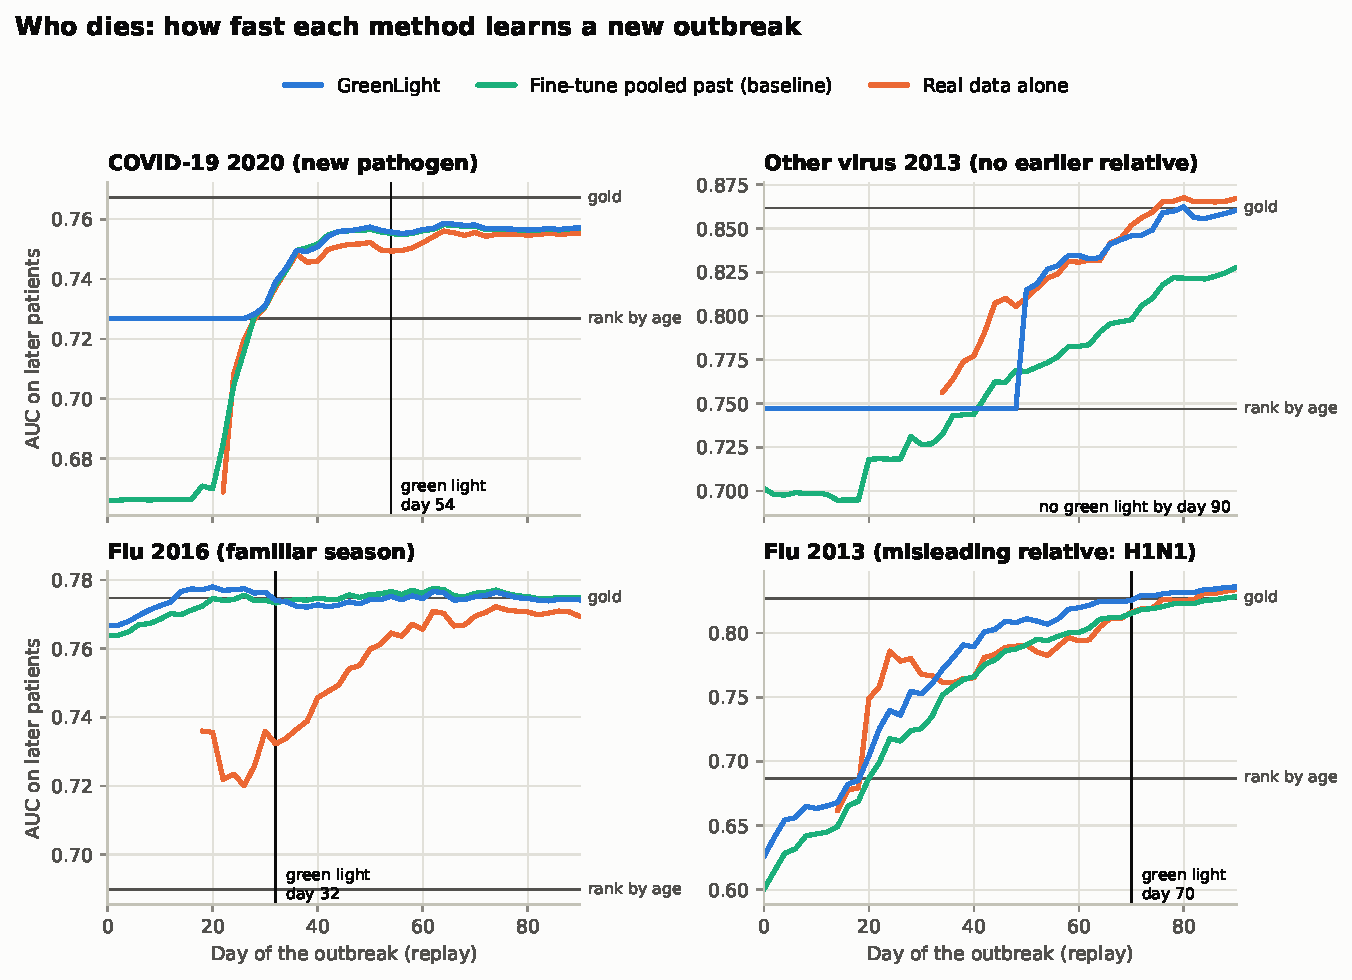
\includegraphics[width=\linewidth]{figures/fig1_replay_curves.pdf}
\caption{AUC on later patients by replay day for four development outbreaks.}\label{fig:replay}
\end{figure}

\begin{table}[t]
\centering\small
\caption{Mean gap to gold over days 0--90 and its difference from GreenLight (positive: GreenLight better), with 95\% paired
bootstrap intervals over outbreaks. Development: 23 outbreaks (2013--2022). Frozen test: 9 outbreaks (2023--2025).}
\label{tab:baselines}
\begin{tabular}{lrrrr}
\toprule
& \multicolumn{2}{c}{Development (23)} & \multicolumn{2}{c}{Frozen test (9)} \\
Method & gap & minus GreenLight & gap & minus GreenLight \\
\midrule
GreenLight & 0.0052 & -- & 0.0067 & -- \\
Real data alone & 0.0520 & +0.047 [0.028, 0.065] & 0.0393 & +0.033 [0.020, 0.046] \\
Pooled earlier outbreaks (no fob data) & 0.0210 & +0.016 [0.003, 0.032] & 0.0010 & $-$0.006 [$-$0.010, $-$0.002] \\
Stacking & 0.0101 & +0.005 [$-$0.002, 0.013] & 0.0006 & $-$0.006 [$-$0.010, $-$0.002] \\
Fine-tuning & 0.0085 & +0.003 [$-$0.001, 0.008] & 0.0070 & +0.000 [$-$0.001, 0.001] \\
GreenLight without the vote & 0.0087 & +0.004 [0.001, 0.006] & 0.0074 & +0.001 [$-$0.000, 0.002] \\
Source averaging & 0.0081 & +0.003 [0.001, 0.005] & 0.0082 & +0.002 [0.001, 0.002] \\
Meta-analytic prior & 0.0140 & +0.009 [0.004, 0.016] & 0.0097 & +0.003 [0.002, 0.004] \\
Robust meta-analytic prior & 0.0166 & +0.011 [0.006, 0.019] & 0.0099 & +0.003 [0.002, 0.004] \\
Empirical-Bayes strength & 0.0146 & +0.009 [0.005, 0.014] & 0.0086 & +0.002 [0.000, 0.004] \\
Meta-learned start & 0.0124 & +0.007 [0.005, 0.010] & 0.0130 & +0.006 [0.003, 0.009] \\
\bottomrule
\end{tabular}
\end{table}

On the development set, GreenLight had the lowest gap, but its margin over stacking and fine-tuning was not distinguishable
from zero; the vote's own contribution (GreenLight versus equal weights) was small but consistent. Every method that borrows
was far better than real data alone. The Lab-Label Fallback mattered most for safety: without it, every borrowing
baseline ranked COVID-19 patients worse than age alone on 24--92 of the first 90 days of 2020, against none for GreenLight
(Figure~\ref{fig:forest}).

\paragraph{Frozen test.} The plan (seasons, settings, endpoints and success criteria) was committed before the
2023--2025 files were downloaded. Five of six criteria held: borrowing beat real data alone; GreenLight never ranked worse
than age; at most one false green light; GreenLight synthetic data beat the real records; no clear gain over fine-tuning.
The sixth failed in the negative direction: \textbf{stacking, and even the pooled earlier seasons with no current
data, were more accurate than GreenLight} (gaps 0.0006 and 0.0010 against 0.0067; GreenLight better in 1 of 9). By 2023 the
history holds many seasons of each pathogen, and season-to-season severity patterns are stable; GreenLight's fixed prior
strength lets a few dozen early records outweigh this history too soon. We did not re-tune GreenLight.

\begin{figure}[t]
\centering
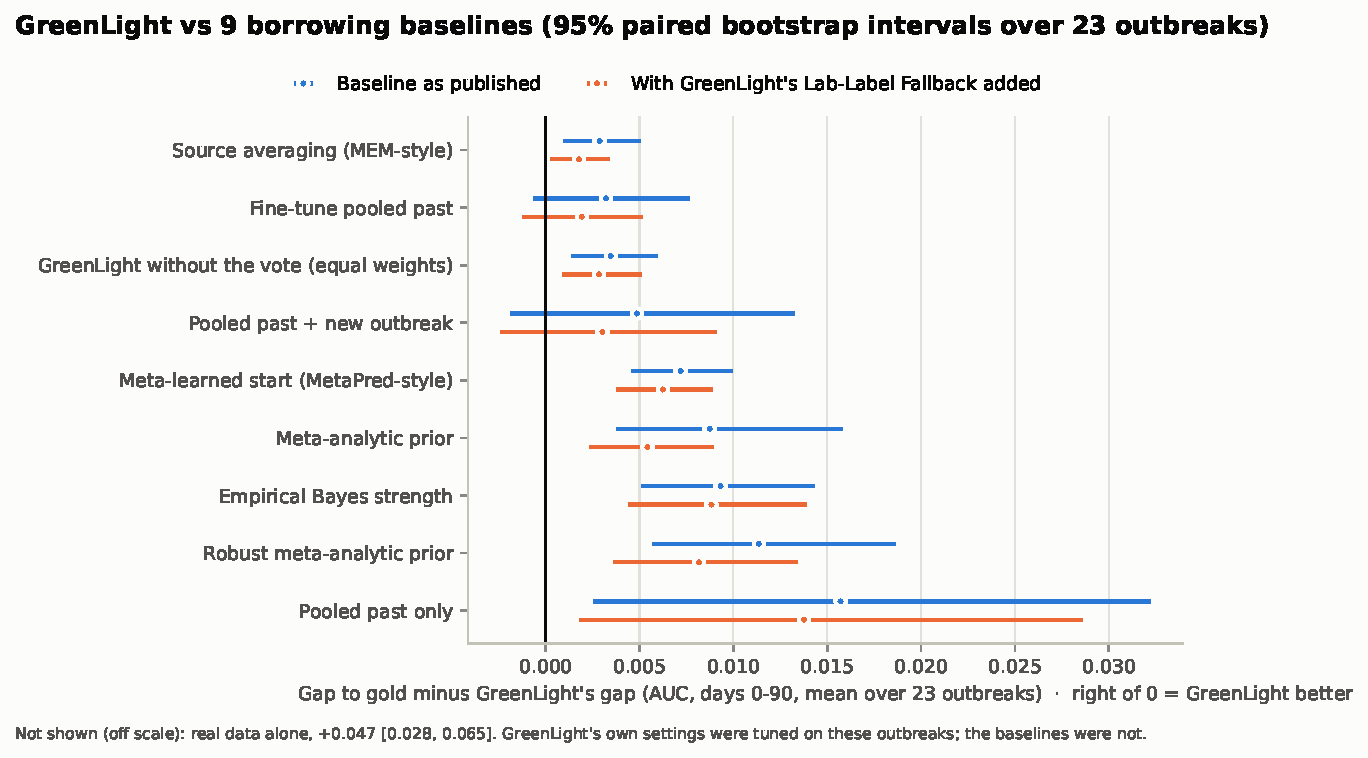
\includegraphics[width=0.85\linewidth]{figures/fig3_baselines_forest.pdf}
\caption{Development set: gap to gold of each baseline minus GreenLight's, with and without GreenLight's Lab-Label Fallback.}\label{fig:forest}
\end{figure}

\paragraph{Calibration.} AUC measures ranking only. Table~\ref{tab:calibration} reports, on the green light day,
whether predicted risks match what happened to the later patients \citep{vancalster2019calibration}. GreenLight's ranking was
well calibrated (slope near 1, unlike real data alone, whose risks were too extreme). Its overall level was right on
average in development but under-predicted deaths by about 15\% on the frozen test; stacking did the same and even the
gold model under-predicted by 9\%, so later patients in those seasons died somewhat more often than earlier ones. The
pooled model, which ignores fob's own death rate, over-predicted deaths by 20--30\%. Brier scores of GreenLight, stacking and
gold were within 0.002 of each other.

\begin{table}[t]
\centering\small
\caption{Calibration on the green light day, scored on the later test patients: mean over outbreaks [95\% bootstrap
interval]. O/E: observed / expected deaths (1 = right level). Slope: logistic recalibration slope (1 = right spread).}
\label{tab:calibration}
\begin{tabular}{lrrrrrr}
\toprule
& \multicolumn{3}{c}{Development (22)} & \multicolumn{3}{c}{Frozen test (9)} \\
Model & O/E & Slope & Brier & O/E & Slope & Brier \\
\midrule
GreenLight & 0.94 [0.84, 1.03] & 0.96 [0.90, 1.01] & 0.097 & 1.15 [1.05, 1.29] & 0.97 [0.92, 1.02] & 0.081 \\
Real data alone & 1.08 [0.93, 1.26] & 0.75 [0.67, 0.84] & 0.105 & 1.08 [0.97, 1.20] & 0.84 [0.75, 0.92] & 0.084 \\
Pooled earlier outbreaks & 0.80 [0.73, 0.87] & 0.89 [0.81, 0.96] & 0.102 & 0.70 [0.58, 0.83] & 1.04 [0.99, 1.09] & 0.082 \\
Stacking & 1.00 [0.90, 1.08] & 0.92 [0.87, 0.97] & 0.098 & 1.15 [1.03, 1.29] & 1.04 [0.99, 1.09] & 0.080 \\
Gold (hindsight) & 1.02 [0.97, 1.08] & 1.29 [1.16, 1.42] & 0.096 & 1.09 [1.03, 1.14] & 1.10 [1.06, 1.15] & 0.080 \\
\bottomrule
\end{tabular}
\end{table}

\subsection{Is the model ready?}\label{sec:readiness}
With the adopted settings (10 deaths, stability 0.99), 22 of 23 development outbreaks turned green by day 90
(median day 38, interval [32, 46]) with no false signal (a model more than 0.02 AUC below gold), and 9 of 9 frozen
test outbreaks (median day 34) with one borderline false signal (other virus 2023, gap 0.021). Choosing the settings
with each development outbreak held out gave one false signal in 22. At the patient level, 22 of 31 green days were
firmly correct, 9 uncertain because small test windows give wide intervals, and none firmly false
(Figure~\ref{fig:readiness}). Riley's minimum sample size \citep{riley2020samplesize}, with the anticipated
$R^2$ taken from the pooled earlier outbreaks, required 2,100--7,100 patients with a known outcome: it declared readiness in
8 of 32 outbreaks (the six COVID-19 seasons and influenza 2016 and 2022) and never for other respiratory
viruses, although for most seasons the borrowed model is near gold from day 0.

\begin{figure}[t]
\centering
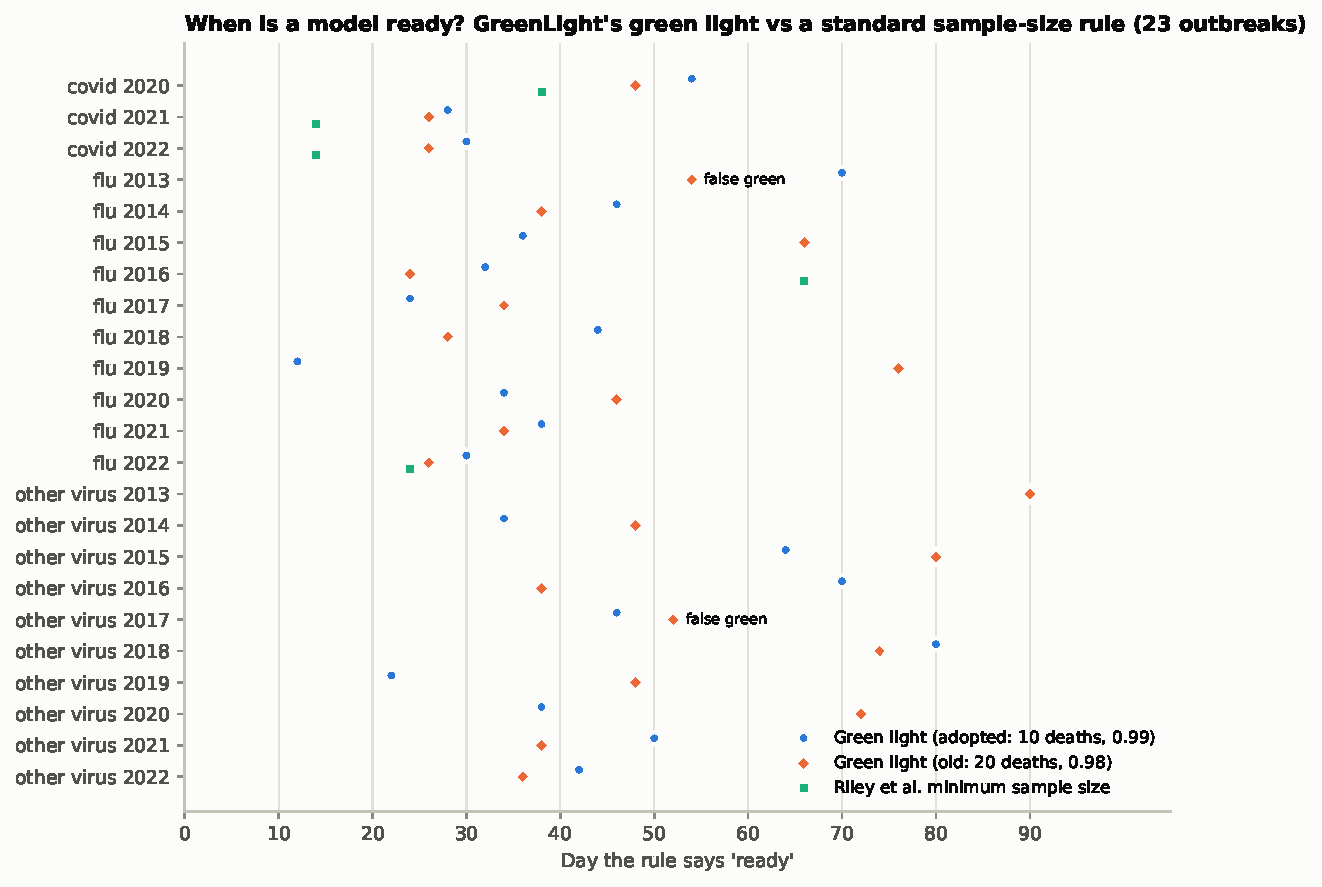
\includegraphics[width=0.85\linewidth]{figures/fig4_readiness.pdf}
\caption{Day each readiness rule declares a model ready, development outbreaks.}\label{fig:readiness}
\end{figure}

\subsection{Which outbreaks does the new one resemble?}
The vote put most weight on the right pathogen group for 19 of 21 development outbreaks with an earlier group member
in weeks 1--4 and 20 of 21 from week 8; on the frozen test, 9 of 9 in every week checked. When the group share was at
least 95\%, it was right 97.6\% of the time. The Stranger took over for COVID-19 in 2020 in week 4, after 3,538
patients (Figure~\ref{fig:votes}); it needs hundreds of patients, so for small outbreaks the laboratory label is the
practical safeguard.

\begin{figure}[t]
\centering
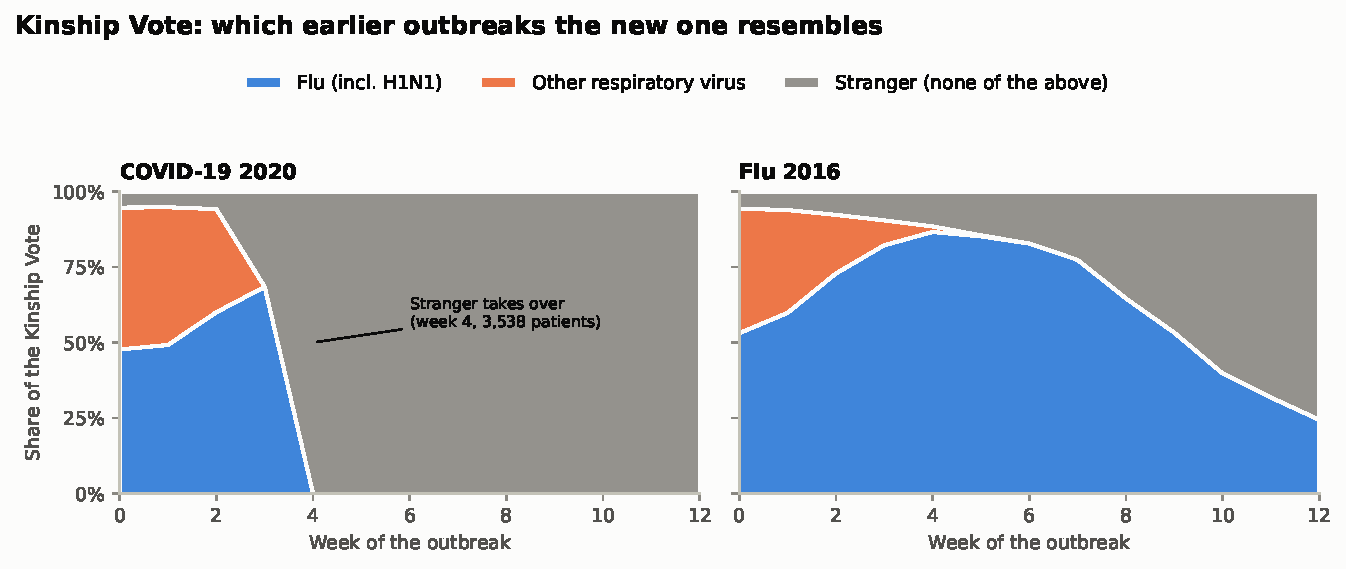
\includegraphics[width=\linewidth]{figures/fig2_kinship_vote.pdf}
\caption{Kinship Vote shares by pathogen group and the Stranger.}\label{fig:votes}
\end{figure}

\subsection{Synthetic data}
On the green light day we trained a ridge logistic model on 50,000 synthetic rows and scored it on the later real
patients (Figure~\ref{fig:synth}). Development: GreenLight synthetic data 0.796 [0.781, 0.811]; the real records it was built
from 0.730; ARF 0.770, TVAE 0.704, bootstrap resampling 0.679, Bayesian network 0.676, CTGAN 0.613, each trained on
those same records. For outbreaks with fewer than 1,000 records, adding GreenLight synthetic rows to the real ones raised AUC
by 0.086 [0.064, 0.109]. Frozen test: GreenLight minus real records +0.035 [0.013, 0.058], minus ARF +0.016 [0.008, 0.024].
TabDDPM \citep{kotelnikov2023tabddpm} could not be run on our CPU budget. The comparison is not like for like by
design: the generators see only fob's records, while GreenLight's data carry borrowed knowledge. The gap shrinks where fob's
own records are plentiful, and in one season (influenza 2022) bootstrap and ARF beat GreenLight.

\paragraph{Copy check.} Records are coarse (age in years, sex, race, state, 16 yes/no fields, outcome), so a genuinely
new patient often matches an earlier one exactly. We therefore compare the share of synthetic rows that exactly match
a record the generator saw with the share of later, unseen real patients that do. GreenLight's synthetic data matched at the
chance level: 12.7\% against 11.4\% (difference +0.013 [$-$0.009, 0.035]) on the development set and 11.3\% against
13.5\% ($-$0.022 [$-$0.052, 0.000]) on the frozen test. Bootstrap resampling, which copies by design, matched 100\%.
This is a check for copying, not a privacy guarantee \citep{stadler2022groundhog}; the source data are public.

\begin{figure}[t]
\centering
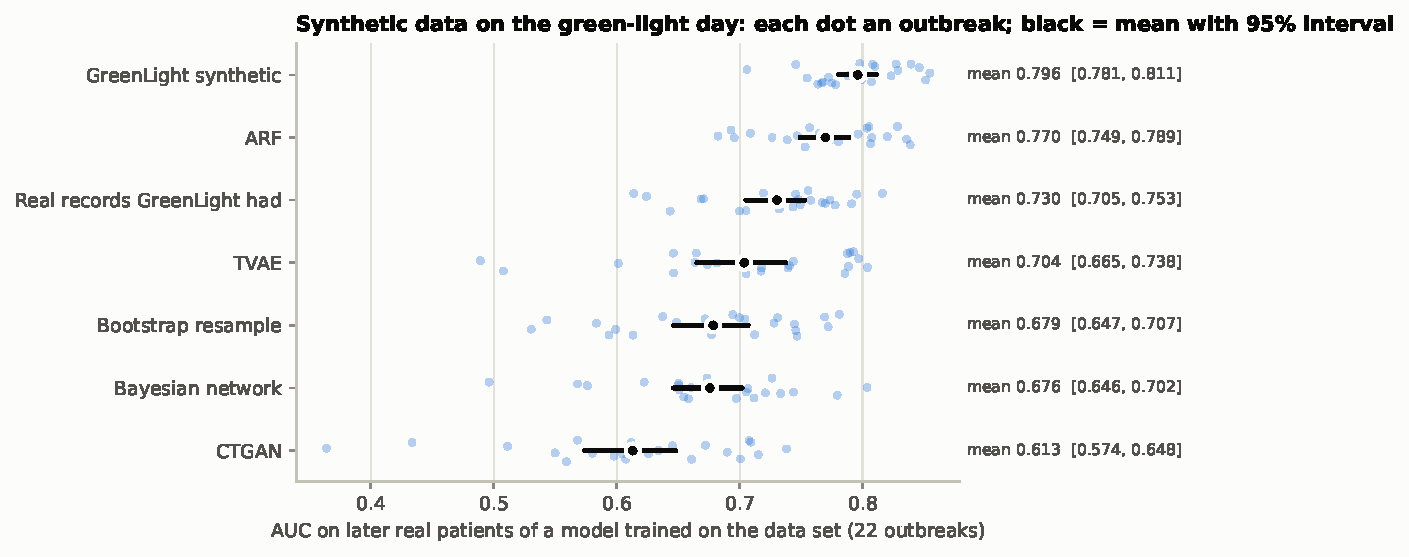
\includegraphics[width=0.9\linewidth]{figures/fig5_synthetic_generators.pdf}
\caption{AUC on later real patients of a model trained only on each data set, development outbreaks.}\label{fig:synth}
\end{figure}

\paragraph{Sensitivity to outcome timing.} Counting an outcome only from the case-closure date, a more cautious
choice, weakened GreenLight slightly on the development set (mean gap 0.0068 against 0.0053; 94 days below age against 66) and
gave one false green light in 22 (other virus 2017; median green day 41 against 38). For COVID-19 in 2020, real data
alone came within 0.02 of gold two days before GreenLight (day 34 against 36). The conclusions do not change.

\section{Discussion}
\paragraph{What GreenLight contributes.} Not a better borrowing formula: plain pooling is a strong, simple competitor and was
better on the frozen test. What held up on unseen seasons is what the baselines lack: a safe fallback for a new
pathogen, a readiness signal that was honest, a vote that found the right group, and synthetic data whose usefulness
comes from borrowed knowledge rather than from the generator.
\paragraph{Why pooling won.} GreenLight lets fob's data take over at a fixed rate. When the history is rich and the new season
familiar, that hands over too soon. A natural fix, letting the borrowing strength grow with the vote's confidence that
fob is familiar, is new development work and needs a new held-out test.
\paragraph{Limitations.} One country and one surveillance system for the main analyses; one truly new pathogen
(COVID-19); admission-form features only; AUC on a later window as the main metric; a fixed ridge model to score
synthetic data. An earlier out-of-country check on Mexico's COVID-19 data used outcome-on-entry timing because
survivors have no outcome date there, and is not reported as evidence. The test outbreaks contain no new pathogen.
\paragraph{Broader impact.} Synthetic records here hold no more information than the real records and the earlier
outbreaks they come from. They are labelled synthetic, must not be presented as real patients, and cannot reveal a
risk factor nobody has recorded.

\section{Reproducibility}
All data are public (CC-BY). Code, pinned environments, configuration files, seeds, the frozen-test plan and a
running results log are available at \PENDING{anonymous code link}. The frozen-test plan was committed before the
test data were downloaded; the commit hash is given in the repository.


\bibliography{refs}
\bibliographystyle{tmlr}

\end{document}
